% !TeX root = ../../V7_Lichtbeugung.tex
\begin{tikzpicture}

\begin{axis}[%
width=0.95\textwidth,
height=0.5\textwidth,
at={(0\textwidth,0\textwidth)},
%scale only axis,
xmin=-5,
xmax=5,
xlabel={$\tfrac{x}{\sigma}$ bzw. $\sigma k$},
ymin=0,
ymax=1,
% ylabel={$y$ bzw. $y \div \sqrt{2\pi}\sigma$}
]
\addplot [samples=500, color=black]
plot (\x, {exp(-pow(\x,2) / 2)});

\addplot [samples=500, color=red]
plot (\x, {exp(-pow(\x,2))});

\end{axis}
\end{tikzpicture}%